\documentclass[12pt]{article}
\usepackage[utf8]{inputenc}

\title{Analysis and Design of Algorithms}
\author{}
\date{April 2019}

\usepackage{natbib}
\usepackage{graphicx}
\usepackage{hyperref}
\usepackage[linguistics]{forest}
\usepackage{tikz}

\usepackage{listings}
\usepackage{xcolor}

\lstdefinestyle{listingcode}
{
    frame             = shadowbox,
    columns           = fullflexible, %Represents the spacing intended (default: fixed; flexible, fullflexible)
    framerule         = 0.1pt, %Thickness of the edge of the box
    framesep          = 2pt, %Separafion of the frame from the text.
    numbers           = left, %Where to put the line-numbers
    rulecolor         = \color{black}, %Box color    
    rulesepcolor      = \color{gray!30}, %Shade color of the box.
}

\begin{document}

\maketitle
\section{Warm up}

Lets modify the classic merge sort algorithm a little bit. What happens if instead of splitting the array in 2 parts we divide it in 3? You can assume that exists a three-way merge subroutine. What is the overall asymptotic running time of this algorithm?

\emph{BONUS:} Implement the three-way merge sort algorithm.

\subsection*{Solution}
The time execution T(n) for three-way merge, where n is the input size. So \textit{T(n)=3T(n/3)+cn}, where \textit{T(n/3)} solves the subproblems through recursive calls and \textit{cn} do the merger in a constant time.\\

We have the next tree for three-way merge:
\begin{center}
\begin{forest}
[n, name = node 1 [n/3, name = node 2 [n/9, name = node 3 [1, edge = dotted, name = node 4]][n/9[1, edge = dotted]][n/9[1, edge = dotted]]]
  [n/3[n/9[1, edge = dotted]][n/9[1, edge = dotted]][n/9[1, edge = dotted]]]
  [n/3[n/9[1, edge = dotted]][n/9[1, edge = dotted]][n/9[1, edge = dotted]]]]
\end{forest}
\end{center}

The top level has total cost \textit{cn}, the next level down has total cost \textit{3c(n/3)=cn}.
In general, each level has total cost \textit{cn}.\\

The total number of levels of the recursion tree is $log_3(n)+1$, where
\textit{n} is the number of leaves, corresponding to the input size. The total time for three-way merge, then, is $cn(log_3(n)+1) = cn*log_3(n)+cn$. When we use big-O notation to describe this running time, we have a running time of $n log_3 n$.

\subsection*{Implementation}
Three Way Merge Sort File = ('cpp/three-way-merge.cpp')

\section{Competitive programming}

Welcome to your first competitive programming problem!!! 

\begin{itemize}
    \item Sign-up in Uva Online Judge (\url{https://uva.onlinejudge.org}) and in CodeChef if you want (we will use it later).
    \item Rest easy! This is not a contest, it is just an introductory problem. Your first problem is located in the ``Problems Section'' and is \textbf{100 - The 3n + 1 problem. $==>$ File: cpp/p100-The3n+1.cpp}
    
    \item Once that you finish with that problem continue with \textbf{458 - The Decoder}. Again, this problem is just to build your confidence in competitive programming. \textbf{ $==>$ File: cpp/p458-TheDecoder.cpp}
    
    \item \emph{BONUS:} \textbf{10855 - Rotated squares $==>$ File: cpp/p10855-RotatedSquares}
    
\end{itemize}
\begin{center}
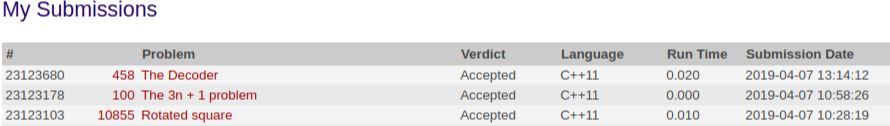
\includegraphics[width=14cm, height=4cm]{img/contest.png}
\end{center}

\section{Simulation}

Write a program to find the minimum input size for which the merge sort algorithm always beats the insertion sort.

\begin{itemize}
    \item Implement the insertion sort algorithm
    \item Implement the merge sort algorithm
    \item Just compare them? No !!! Run some simulations or tests and find the average input size for which the merge sort is an asymptotically ``better'' sorting algorithm.
\end{itemize}

Note: Include (.tex) and attach(.cpp) your source code and use a dockerfile to interact with python and plot your results.\\

\emph{BONUS:} Compare both algorithms against any other sorting algorithm

\subsection{Insertion Sort}
\begin{lstlisting}[language=C++]
#include <iostream>
#include <vector>

using namespace std;

void InsertionSort(vector<int> &list){
    if(list.size()>1){
        int key;
        for(int i = 1; i < list.size(); i++){
            key = list[i];
            int j = i-1;
            while(j >= 0 && list[j] > key){
                list[j+1] = list[j];
                j--;
            }
            list[j+1] = key;
        }
    }
}
\end{lstlisting}

\subsection{Merge Sort}

\begin{lstlisting}[language=C++]
#include <iostream>
#include <vector>

using namespace std;

void Merge(vector<int>vector1,vector<int>vector2,vector<int>&vectorMerge){
    vectorMerge.clear();
    long int pos1 = 0, pos2 = 0;
        while(pos1 < vector1.size() && pos2 < vector2.size()){
        if(vector1[pos1]<vector2[pos2]){
            vectorMerge.push_back(vector1[pos1]);
            pos1++;
        }
        else{
            vectorMerge.push_back(vector2[pos2]);
            pos2++;
        }
    }

    while (pos1<vector1.size()) {
        vectorMerge.push_back(vector1[pos1]);
        pos1++;
    }
    while (pos2<vector2.size()) {
        vectorMerge.push_back(vector2[pos2]);
        pos2++;
    }
}

void MergeSort(vector<int> &list){
    if(list.size()>1) {
        vector<int> first, second;
        for (long int i = 0; i < list.size() / 2; i++)
            first.push_back(list[i]);
        for (long int i = (list.size() / 2); i < list.size(); i++)
            second.push_back(list[i]);

        MergeSort(first);
        MergeSort(second);

        Merge(first, second, list);
    }
}
\end{lstlisting}

\section{Research}

Everybody at this point remembers the quadratic ``grade school'' algorithm to multiply 2 numbers of $k_{1}$ and $k_{2}$ digits respectively. \\

Your assignment now is to compare the number of operations performed by the quadratic grade school algorithm and Karatsuba multiplication.

\begin{itemize}
    \item Define Karatsuba multiplication
    \item Implement grade school multiplication
    \item Implement Karatsuba multiplication
    \item Compare Karatsuba algorithm against grade school multiplication
    \item Use any of your implemented algorithms to multiply $a*b$ where:
    \begin{description}
    \item{a:} 3141592653589793238462643383279502884197169399375105820974944592
    \item{b:} 2718281828459045235360287471352662497757247093699959574966967627
    \end{description}
\end{itemize}

Note: Include(.tex) and attach(.cpp) your source code, of course.\\

\emph{BONUS:} How about Sch\"{o}nhage-Strassen algorithm ? 

\subsection*{Karatsuba multiplication}

Given two numbers, x and y, represented as n-digits strings. For $m < n (m = n/2$ is most efficient).
\\
We have :
\begin{center}
    $x_1, x_0: x = x_1 10^m+x_0$ and $y_1, y_0; y = y_1 10^m+y_0$ ; $x,y<10^m$.
\end{center}
And the product is
\begin{center}
    $xy = (x_1 10^m+x_0)(y_1 10^m+y_0)$\\
    $xy = z_2 10^{2m}+z_1 10^m + z_0$
\end{center}
Where:
\begin{center}
    $z_2 = x_1y_1,$
    $z_1 = x_1y_0+x_0y_1,$
    $z_0 = x_0y_0.$
\end{center}
And we can observe that:
\begin{center}
    $z_1=(x_1+x_0)(y_1+y_0)-z_2-z_0$
\end{center}
When we use the algorithm, we have to solve three smaller multiplications. If n is two or more, those products can be computed by recursive calls of the algorithm.
\subsection*{Implementations}
Grade School File: cpp/gsm.cpp\\
Karatsuba File: cpp/Karatsuba.cpp

\subsection*{Comparison}
For any $n>1$, the number of single-digit multiplications is at most $3n^{lg3}$. Then:
\begin{center}
    $T(n)=3T(n/2)+cn$
\end{center}
Where, $3T(n/2)$ represents the three multiplications of the two separations of the number and $cn$ is the time proportional it takes to execute the additions, subtractions and digits shifts.
This algorithm gives: $T(n)=O(n^{lg3})$, that is faster than grade school multiplication $O(n^2)$.

\begin{center}
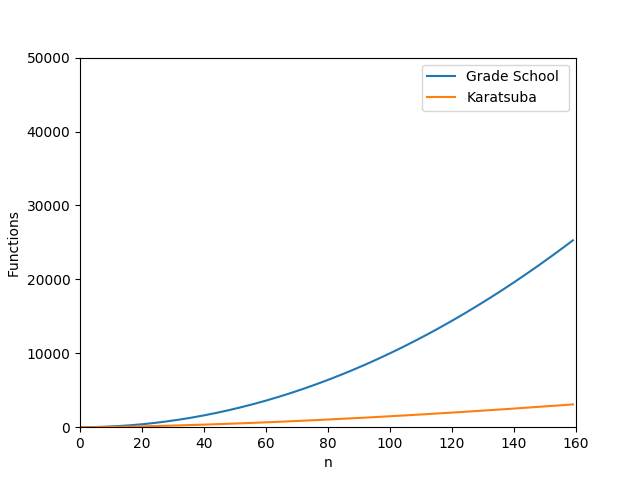
\includegraphics[]{img/Figure_2.png}

\end{center}

\subsection*{Exercise}

With Grade School Multiplication with:
\begin{description}
    \item{a:} 3141592653589793238462643383279502884197169399375105820974944592
    \item{b:} 2718281828459045235360287471352662497757247093699959574966967627
    \item{a*b=} 85397342226735670654635508695465744950348885357651149618796011\\
    27067743044893204848617875072216249073013374895871952806582723184
    \end{description}

\section{Wrapping up}

Arrange the following functions in increasing order of growth rate with $g(n)$ following $f(n)$ if $f(n) = \mathcal{O}(g(n))$

\begin{enumerate}
    \item $n^{2}log(n)$
    \item $2^{n}$
    \item $2^{2^{n}}$
    \item $n^{log(n)}$
    \item $n^{2}$
\end{enumerate}

\begin{center}
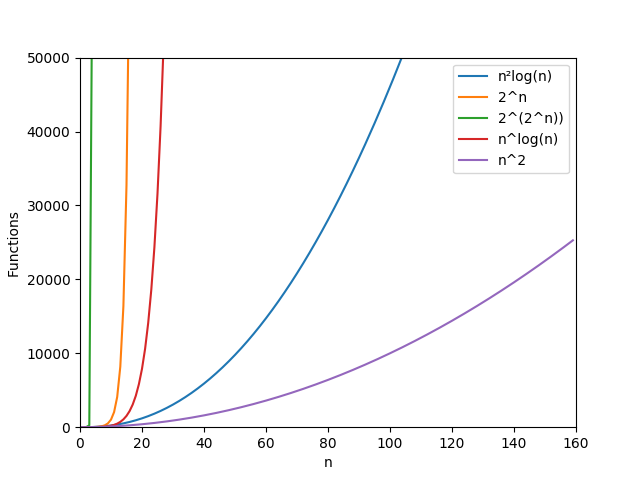
\includegraphics[width=15cm, height=6cm]{img/Figure_1.png}
\end{center}

Functions in order:

\begin{enumerate}
    \item $n^{2}$
    \item $n^{2}log(n)$
    \item $n^{log(n)}$
    \item $2^{n}$
    \item $2^{2^{n}}$
\end{enumerate}

\end{document}